\documentclass[8pt]{exam} 
 \renewcommand{\thesubpart}{(\roman{subpart})}
 \renewcommand{\subpartlabel}{\thesubpart}
 \footer{}{}{Page \thepage\ de \numpages}
\addpoints
% \pointsinmargin
% \boxedpoints
\renewcommand{\questionshook}{\setlength{\itemsep}{1mm}}
\renewcommand{\partshook}{
	\setlength{\itemsep}{0.1cm}
}


\usepackage{cmbright}

\pagestyle{empty} %for handouts
\addtolength{\jot}{2em} % this makes all formulae a bit more spaced vertically for handouts
\setlength{\parindent}{0pt} %we're not writing a novel
%\renewcommand{\arraystretch}{2} %makes tables taller, so easier to write in

\usepackage[fleqn]{amsmath}
\usepackage{amssymb} %standard classy maths symbols
\usepackage[a4paper, margin=1in]{geometry} %makes it easy to specify where to put stuff on the page

\usepackage[utf8]{inputenc}

\usepackage{tcolorbox} % basic but good package for boxes around text
\tcbset{colback=black!2!white}


\usepackage{tikz}

\begin{document}

\textbf{Name:} \makebox[8cm]{\dotfill}

\vspace{-3mm}

\begin{minipage}{0.55\textwidth}
\textbf{Without calculator}

\

On the unit circle, define $A = P(\frac{\pi}{6})$ and $B = P(-\frac{\pi}{6})$. \\
As usual $O$ denotes the origin, $(0; 0)$.

\

See the diagram to the right.



\end{minipage}
\begin{minipage}{0.35\textwidth}
\vspace{0mm}
\begin{center}
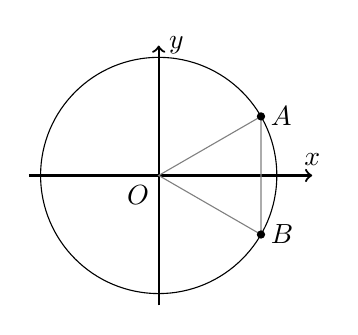
\begin{tikzpicture}[scale=1.5]
%\clip (-14,-4.2) rectangle (14.5,4.7);
%\draw[help lines, step=1, white!50!gray] (-14.1,-14.1) grid (14.1,14.1);
%\draw[help lines,line width=.8pt,step=1] (-0.1,-0.1) grid (10.1,10.1);

\draw[thick, ->] (-1.1,0) -- (1.3,0) node[above] {$x$};
\draw[thick, ->] (0,-1.1) -- (0,1.1) node[right] {$y$};

% Curve
\draw (0,0) circle (1cm);
\draw[gray] (0.866, -0.5) -- (0,0) node[below left, black] {$O$} -- (0.866, 0.5) -- cycle;

\draw[fill, black] (0.866, 0.5) circle (0.3mm) node[right] {$A$};
\draw[fill, black] (0.866, -0.5) circle (0.3mm) node[right] {$B$};

\end{tikzpicture}
\end{center}
\end{minipage}

\begin{questions}


\question[1] Explain why $\overline{OA} = 1$
\fillwithdottedlines{7mm}

\question[1] Let $M$ be the midpoint of the segment $[AB]$. Explain why $M\hat{O}A = \frac{\pi}{6}$.
\fillwithdottedlines{7mm}

\question[1] Sketch $\triangle MOA$ and label the angle $M\hat{O}A$. Then label the sides of this right-angled triangle (hyp; adj; opp).
\vspace{25mm}

\question[1] Explain why $\triangle OAB$ is an equilateral triangle and give the length $\overline{AM}$.
\fillwithdottedlines{28mm}


\question[1] Let $a = \overline{OM}$. Using Pythagoras in $\triangle MOA$ calculate $a$ as an exact value.
\fillwithdottedlines{21mm}

\question[1] Hence, using the definition of cosine, calculate $\cos(\frac{\pi}{6})$ as an exact value.
\fillwithdottedlines{21mm}

\question[0] \textbf{Bonus.} Solve the equation $\sin \theta = \frac{1}{2}$. \hfill \emph{Work on the back.}



\end{questions}
\vfill 

\begin{tcolorbox}

\textbf{Name of corrector:}

\begin{center}
\gradetable[h][questions]
\end{center}

\end{tcolorbox}


\end{document}